\documentclass[8pt]{extarticle}
\title{}
\author{Avinash Iyer}
\date{}

%font setup
%
%\usepackage[math]{anttor}

%paper setup
\usepackage{geometry}
\geometry{letterpaper, portrait, margin=1in}
\usepackage{fancyhdr}

%symbols
\usepackage{amsmath}
\usepackage{amssymb}
\usepackage{hyperref}
\usepackage{gensymb}

\usepackage[T1]{fontenc}
\usepackage[utf8]{inputenc}

%chemistry stuff
\usepackage[version=4]{mhchem}
\usepackage{chemfig}

%plotting
\usepackage{pgfplots}
\usepackage{tikz}

%\usepackage{natbib}

%graphics stuff
\usepackage{graphicx}
\graphicspath{ {./images/} }

%a useful command
\newcommand{\plain}[1]{\textrm{#1}}

%code stuff
%when using minted, make sure to add the -shell-escape flag
%you can use lstlisting if you don't want to use minted
%\usepackage{minted}
%\usemintedstyle{pastie}
%\newminted[javacode]{java}{frame=lines,framesep=2mm,linenos=true,fontsize=\footnotesize,tabsize=3,autogobble,}
%\newminted[cppcode]{cpp}{frame=lines,framesep=2mm,linenos=true,fontsize=\footnotesize,tabsize=3,autogobble,}

\usepackage{listings}
\usepackage{color}
\definecolor{dkgreen}{rgb}{0,0.6,0}
\definecolor{gray}{rgb}{0.5,0.5,0.5}
\definecolor{mauve}{rgb}{0.58,0,0.82}

\lstset{frame=tb,
	language=Java,
	aboveskip=3mm,
	belowskip=3mm,
	showstringspaces=false,
	columns=flexible,
	basicstyle={\small\ttfamily},
	numbers=none,
	numberstyle=\tiny\color{gray},
	keywordstyle=\color{blue},
	commentstyle=\color{dkgreen},
	stringstyle=\color{mauve},
	breaklines=true,
	breakatwhitespace=true,
	tabsize=3
}
% text + color boxes
\usepackage{tcolorbox}
\newtcolorbox{mathbox}[1]{title = {#1}}

\pagestyle{fancy}
\fancyhf{}
\rhead{Avinash Iyer}
\lhead{Problem Set 1}
\begin{document}
\section*{Growth and Development}%
\subsection*{Part A}
  \begin{quote}
    In 2017, Ethiopia had a per capita income of \$1600, or about \$4 per day. Compute per capita income in Ethiopa 50 years down the line, assuming four different average annual growth rates of 1\%, 2\%, 4\%, and 6\%. Do your results indicate that small differences in growth rates have large effects over time?
  \end{quote}
    \begin{align*}
      Y_{1} &= 1600\cdot (1.01)^{50} \\
          &= 2631 \\
      Y_{2} &= 1600 \cdot (1.02)^{50} \\
          &= 4360\\
      Y_{3} &= 1600\cdot (1.04)^{50}\\
          &= 11370\\
      Y_{4} &= 1600 \cdot (1.06)^{50} \\
          &= 29472
    \end{align*}
  This finding supports the fact that small differences in the growth rate of a country can vastly increase overall well-being down the road.
  \subsection*{Part B}%
    \begin{quote}
      The following table shows the per capita GDP (measured in constant 2011 dollars) for three countries in 1980 and 2017. Compute the annual average growth rate of per capita GDP for each country. Which country had the largest average annual rate of economic growth? Which had the smallest?
    \end{quote}
To calculate average annual growth rate, I used the CAGR formula, $\left(\frac{Y_{\textrm{final}}}{Y_{\textrm{initial}}}\right)^{1/t}-1$.
    \begin{center}
      \begin{tabular}{c|cc|c}
        Country & 1980 & 2017 & Average Annual Growth Rate\\
        \hline
        United States & 29219 & 54087 & 1.6\%\\
        China & 826 & 15288 & 8.2\% \\
        India & 1169 & 6420 & 4.7\%
      \end{tabular}
    \end{center}
    According to this table, we can see that the fastest growing country was China at 8.2\% annual growth, while the United States was the slowest growing country at 1.6\% annual growth.
\section*{Ratio Scale}%
  \begin{quote}
    Plot per capita GDP on a ratio scale (with tick marks on the vertical axis that double) between the years 2015 and 2133, based on the following scenario:
      \begin{itemize}
        \item Per capita GDP in the year 2015 is equal to \$10000
        \item Per capita GDP grows at 2\% per year between 2015 and 2085 % in 2050, per capita GDP = 20K, 2085 per capita GDP = 40K
        \item For the next 20 years, per capita GDP grows at 7\% per year % 2095 per capita GDP = 80K, 2105 per capita GDP = 160K
        \item For the next 28 years, per capita GDP growth slows to 5\% per year % 2119 per capita GDP = 320K, 2133 per capita GDP = 640K
      \end{itemize}
  \end{quote}
  \begin{center}
      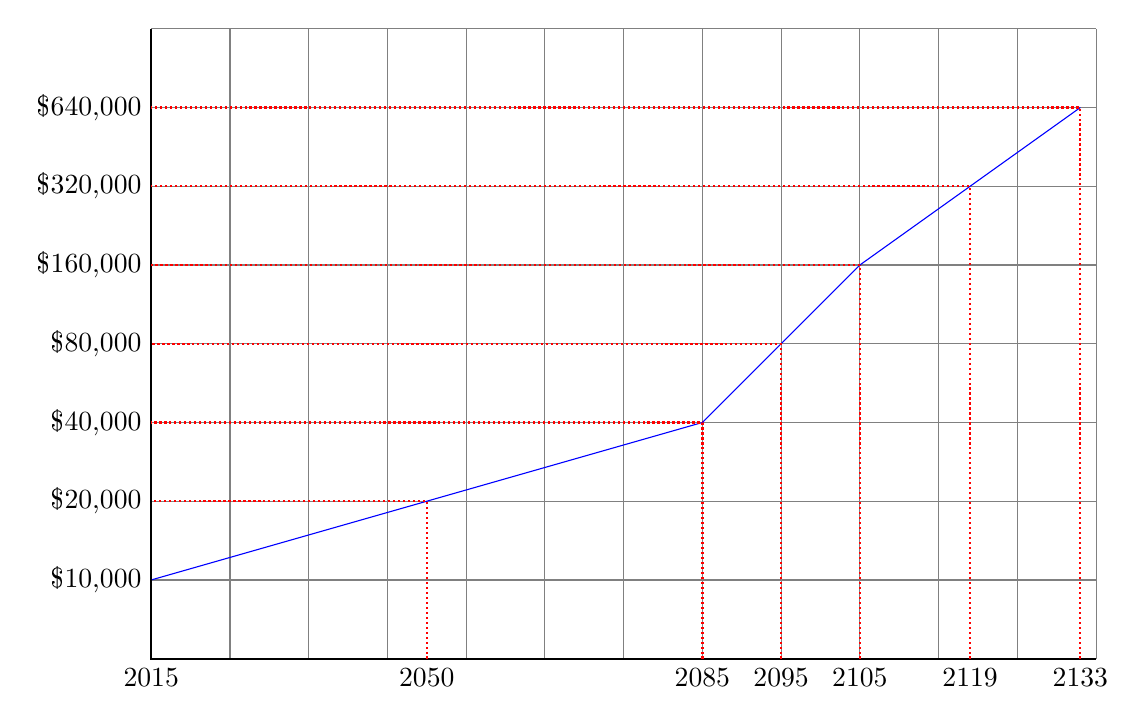
\begin{tikzpicture}
        \draw[step = 1, gray, thin] (0,0) grid (12,8);
        \draw[blue] (0,1) -- (7,3);
        \draw[thick] (0,8) -- (0,0) -- (12,0);
        \node[anchor = north] at (0,0){2015};
        \node[anchor = east] at (0,1) {\$10,000};
        \node[anchor = north] at (3.5,0) {2050};
        \node [anchor=east] at (0,2) {\$20,000};
        \draw[densely dotted, red, thick] (3.5,0) -- (3.5,2) -- (0,2);
        \node[anchor = north] at (7,0) {2085};
        \node[anchor = east] at (0,3) {\$40,000};
        \draw[densely dotted, red, thick] (7,0) -- (7,3) -- (0,3);

        \draw[blue] (7,3) -- (9,5);
        \node[anchor = north] at (8,0) {2095};
        \node[anchor = east] at (0,4) {\$80,000};
        \draw[densely dotted, red , thick] (8,0) -- (8,4) -- (0,4);
        \node[anchor = north] at (9,0) {2105};
        \node[anchor = east] at (0,5) {\$160,000};
        \draw[densely dotted, red, thick] (9,0) -- (9,5) -- (0,5);

        \draw[blue] (9,5) -- (11.8,7);
        \node[anchor = north] at (10.4,0) {2119};
        \node[anchor = east] at (0,6) {\$320,000};
        \draw[densely dotted, red, thick] (10.4,0) -- (10.4,6) -- (0,6);
        \node[anchor = north] at (11.8,0) {2133};
        \node[anchor = east] at (0,7) {\$640,000};
        \draw[densely dotted, red ,thick] (11.8,0) -- (11.8,7) -- (0,7);
      \end{tikzpicture}
  \end{center}
\section*{Computing Growth Rates}%
  \begin{quote}
    Suppose $x = (1.04)^t$ and $y = (1.02)^t$. Calculate the growth rate in each of the following cases.
  \end{quote}
  \begin{itemize}
    \item $z = xy$: $g_z = g_x + g_y = 6\%$
    \item $z = x/y$: $g_z = g_x - g_y = 2\%$
    \item $z = y/x$: $g_z = g_y - g_x = -2\%$
    \item $z = x^{1/2}y^{1/2}$: $g_z = (1/2)g_x + (1/2)g_y = 3\%$
    \item $z = (x/y)^2$: $g_z = 2(g_x-g_y) = 4\%$
    \item $z = x^{-1/3}y^{2/3}$: $g_z = (-1/3)g_x + (2/3)g_y = 0\%$
  \end{itemize}
\section*{True/False}%
  \begin{quote}
    Evaluate the following statement and explain why it is or is not true:
      \begin{quote}
        The growth rate of a product is the sum of the individual growth rates.
      \end{quote}
  \end{quote}
This statement is correct, which we can see through the following:
  \begin{align*}
    x &= (1+g_x)^t \\
    y &= (1+g_y)^t \\
    z &= xy \\
    (1+g_z)^t &= (1+g_x)^t(1+g_y)^t \\
    \ln\left((1+g_z)^t\right) &= \ln\left((1+g_x)^t(1+g_y)^t\right)\\
    t(1+g_z) &= t(1+g_x) + t(1+g_y) \\
    g_z &= g_x + g_y
  \end{align*}
\end{document}
